
% ════════════════════════════════════════════
% 模型求解（5.2.4.模型求解.tex，三级子块）
% ════════════════════════════════════════════
\subsubsection{全年结果与预测精度检验}

按“先预测、再决策、后结算”的三段式结构逐日推进：每天 0:00 由扩张窗口预报模型给出当天 144 个间隔的负载与光伏预测值，据此求解两阶段随机线性规划得到计划购电量与储能充放电计划；当天实际功率到达后，储能按既定计划执行，按式(\ref{eq:q2_delta})结算紧急购电量、按式(\ref{eq:q2_curtail})统计弃电量；日末储电量作为状态传递至次日。2025 年 1 月作为\textbf{预测模型标定期与预热期}：1 月 1 日 0:00 储电量由附录给定为 6000 kWh，此后逐日滚动，至 2 月 1 日 0:00 储电量已收敛至 1200 kWh 下限。按附件 5 口径，结果文件与费用汇总均只统计 2025 年 2 月 1 日至 12 月 31 日共 \textbf{334 天}。

该口径下的全年费用构成为：\textbf{计划购电量 21833065.92 kWh，计划购电费 13325494.59 元；紧急购电量 282910.68 kWh，紧急购电费 1057398.40 元；合计购电费 14382892.99 元}，日均约 43062.55 元，紧急购电量占计划购电量的 1.30\%。334 天中共有 333 天出现紧急购电（占 99.70\%），全年 144$\times$334 个间隔中有 8609 个间隔出现紧急购电（占 17.90\%），最大紧急购电功率 2143.48 kW，单日最大紧急购电量 12595.53 kWh。可见在 0:00 信息不完备的前提下，紧急购电并非偶发事件，而是每天都会发生、但总量很小（约 1\%）的“兜底”电量，这正是 5 倍电价下随机规划给出的经济最优解。

按题目要求，以题目表 1 的格式给出四个指定日期在指定时间段的计划购电量及全天购电量与购电费（表\ref{tab:结果2-1a}$\sim$表\ref{tab:结果2-1d}），以题目表 2 的格式给出指定时间段的充放电量及 0:00 与 24:00 储电量（表\ref{tab:结果2-2a}$\sim$表\ref{tab:结果2-2d}），以题目表 3 的格式给出紧急购电的分段明细（表\ref{tab:结果2-3}）；完整结果已写入 \texttt{result2.xlsx} 的三张工作表。

首先检验预测段的精度。以 334 天全部 144 个间隔的真实值与预测值比对（样本 24222 个），负载预测的平均绝对误差为 130.24 kW、均方根误差为 179.00 kW，相对误差标准差 4.50\%；光伏预测的平均绝对误差为 150.94 kW、均方根误差为 305.54 kW，相对误差标准差 9.95\%。负载的相对误差分位数（$5\%,10\%,\dots,95\%$）为 $-32.32\%$、$-4.68\%$、$-2.86\%$、$-1.75\%$、$-0.87\%$、$-0.06\%$、$0.75\%$、$1.63\%$、$2.78\%$、$4.68\%$、$39.78\%$，即中间 $90\%$ 的间隔误差落在 $-5\%\sim5\%$ 以内，仅夜间负荷极低时（分母很小）出现较大相对偏差；光伏的对应分位数为 $-79.31\%$、$-11.14\%$、$-7.21\%$、$-4.45\%$、$-2.25\%$、$-0.16\%$、$1.86\%$、$4.15\%$、$6.97\%$、$11.37\%$、$95.36\%$，中间 $80\%$ 的间隔误差在 $-11\%\sim11\%$ 以内，两端的极端值同样出现在日出、日落前后光伏出力接近零的时段。预测与实际功率的逐点对比见图\ref{fig:结果2-7}，相对误差分布见图\ref{fig:结果2-8}。

\begin{figure}[H]
    \centering
    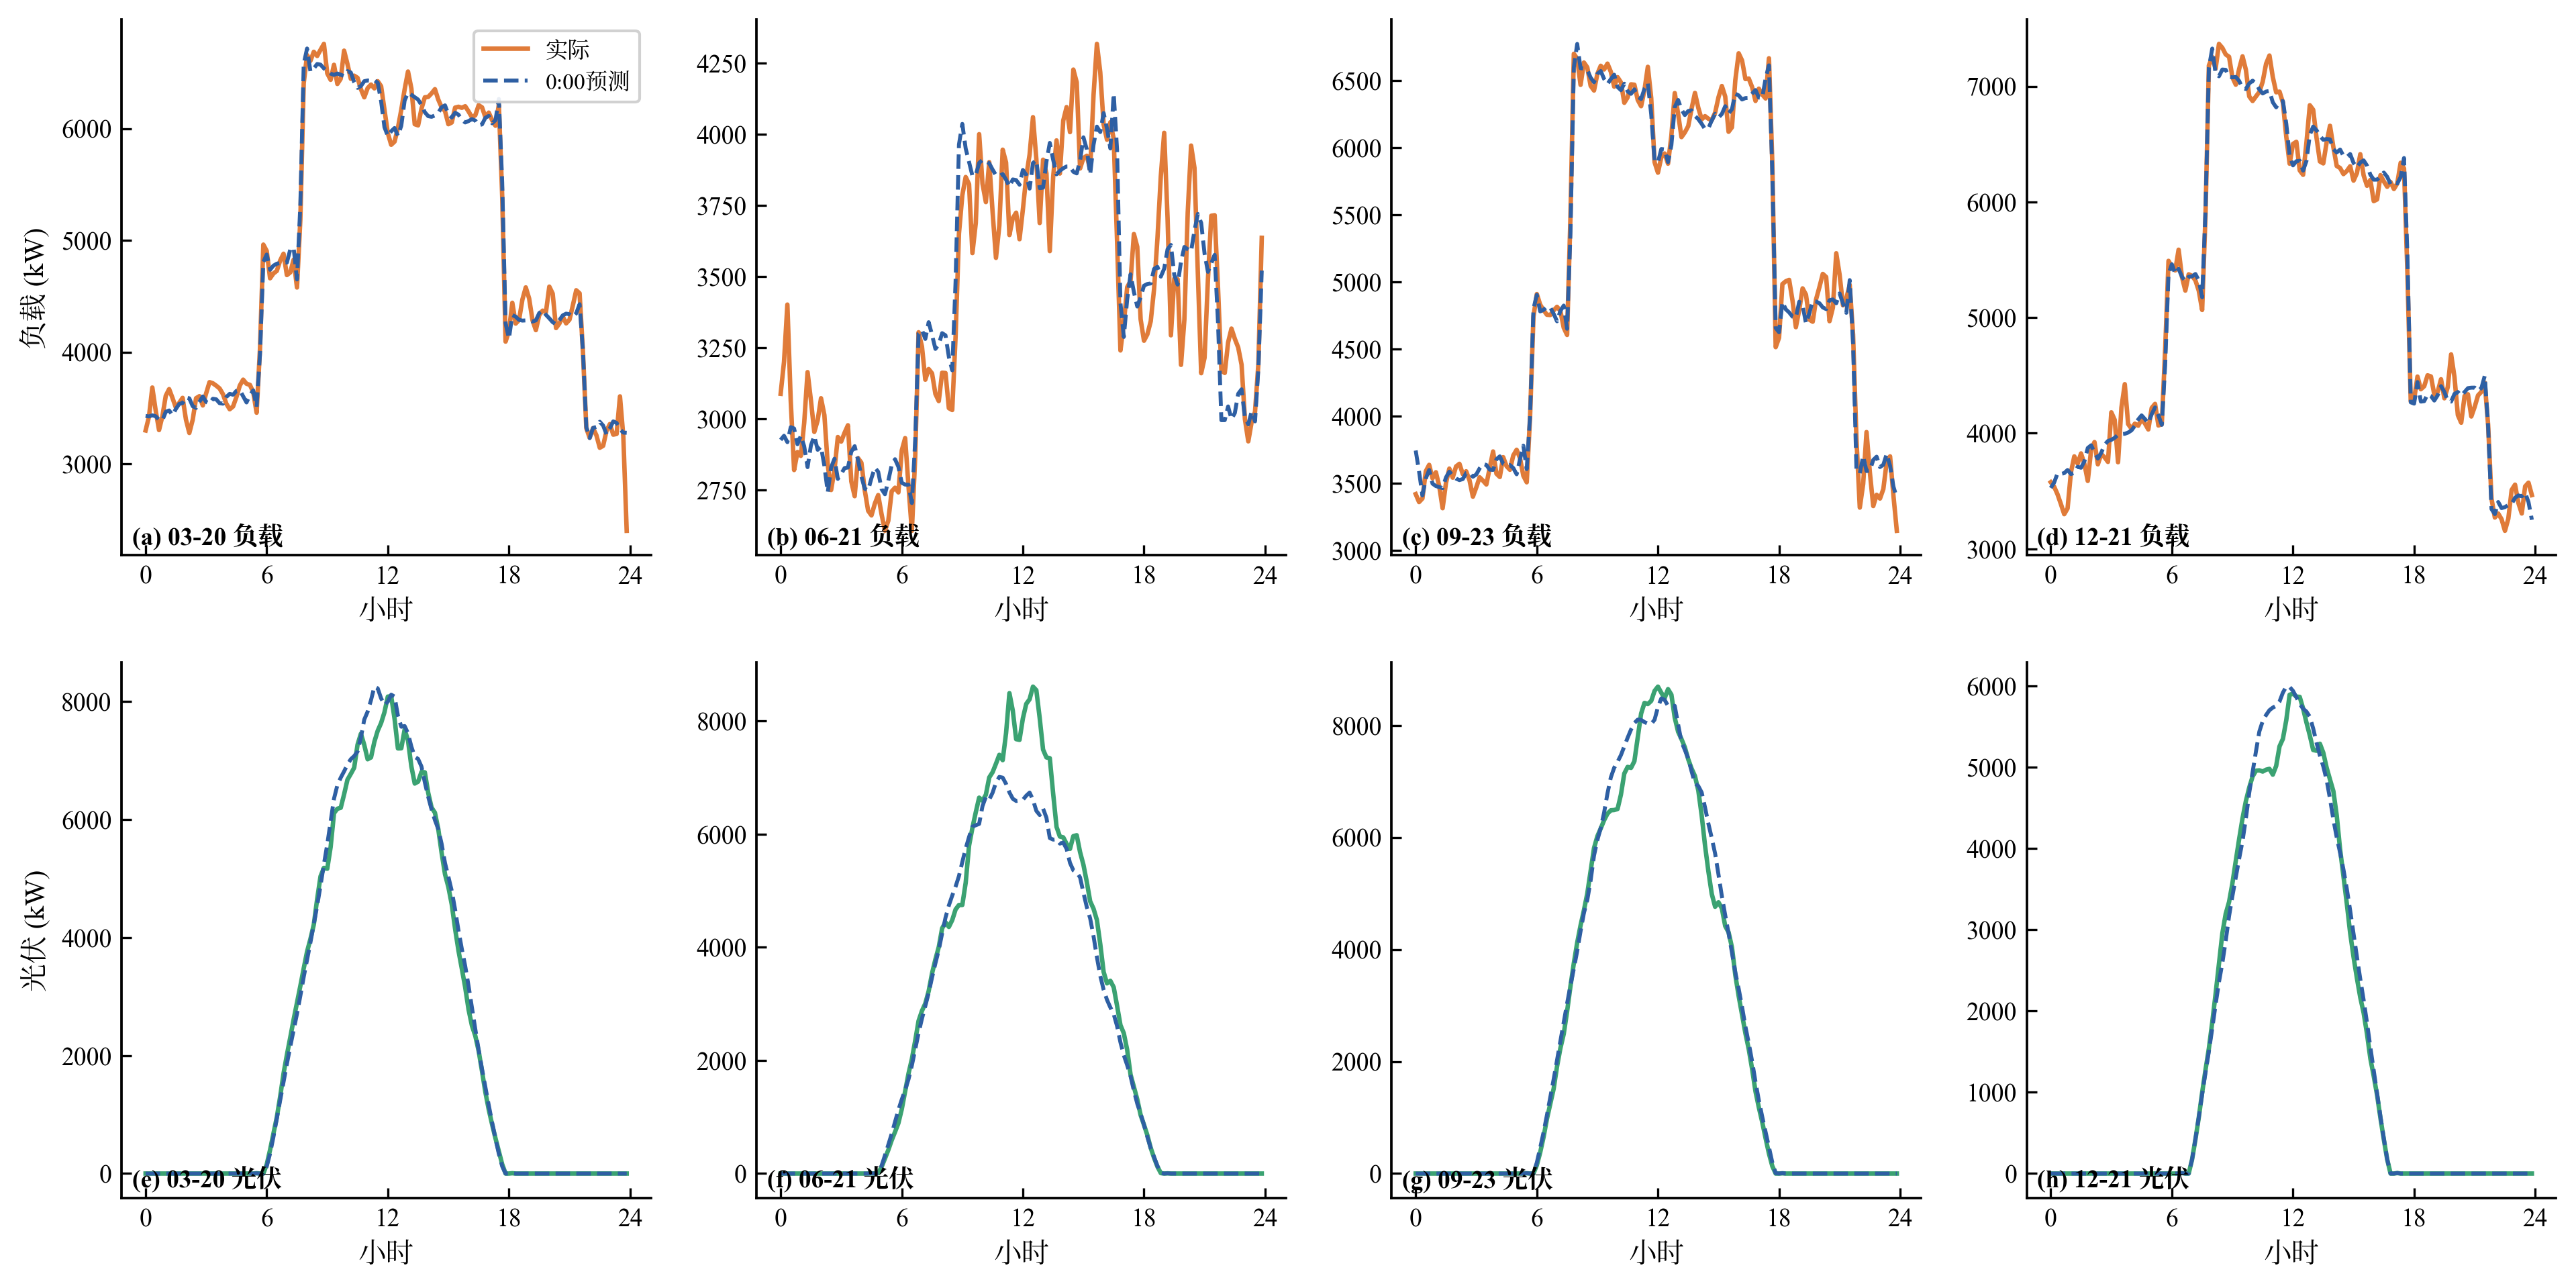
\includegraphics[width=0.78\textwidth]{求解/问题二/图片/图2-7_预测与实际对比.png}
    \caption{典型日负载与光伏的预测值与实际值对比}
    \label{fig:结果2-7}
\end{figure}

\begin{figure}[H]
    \centering
    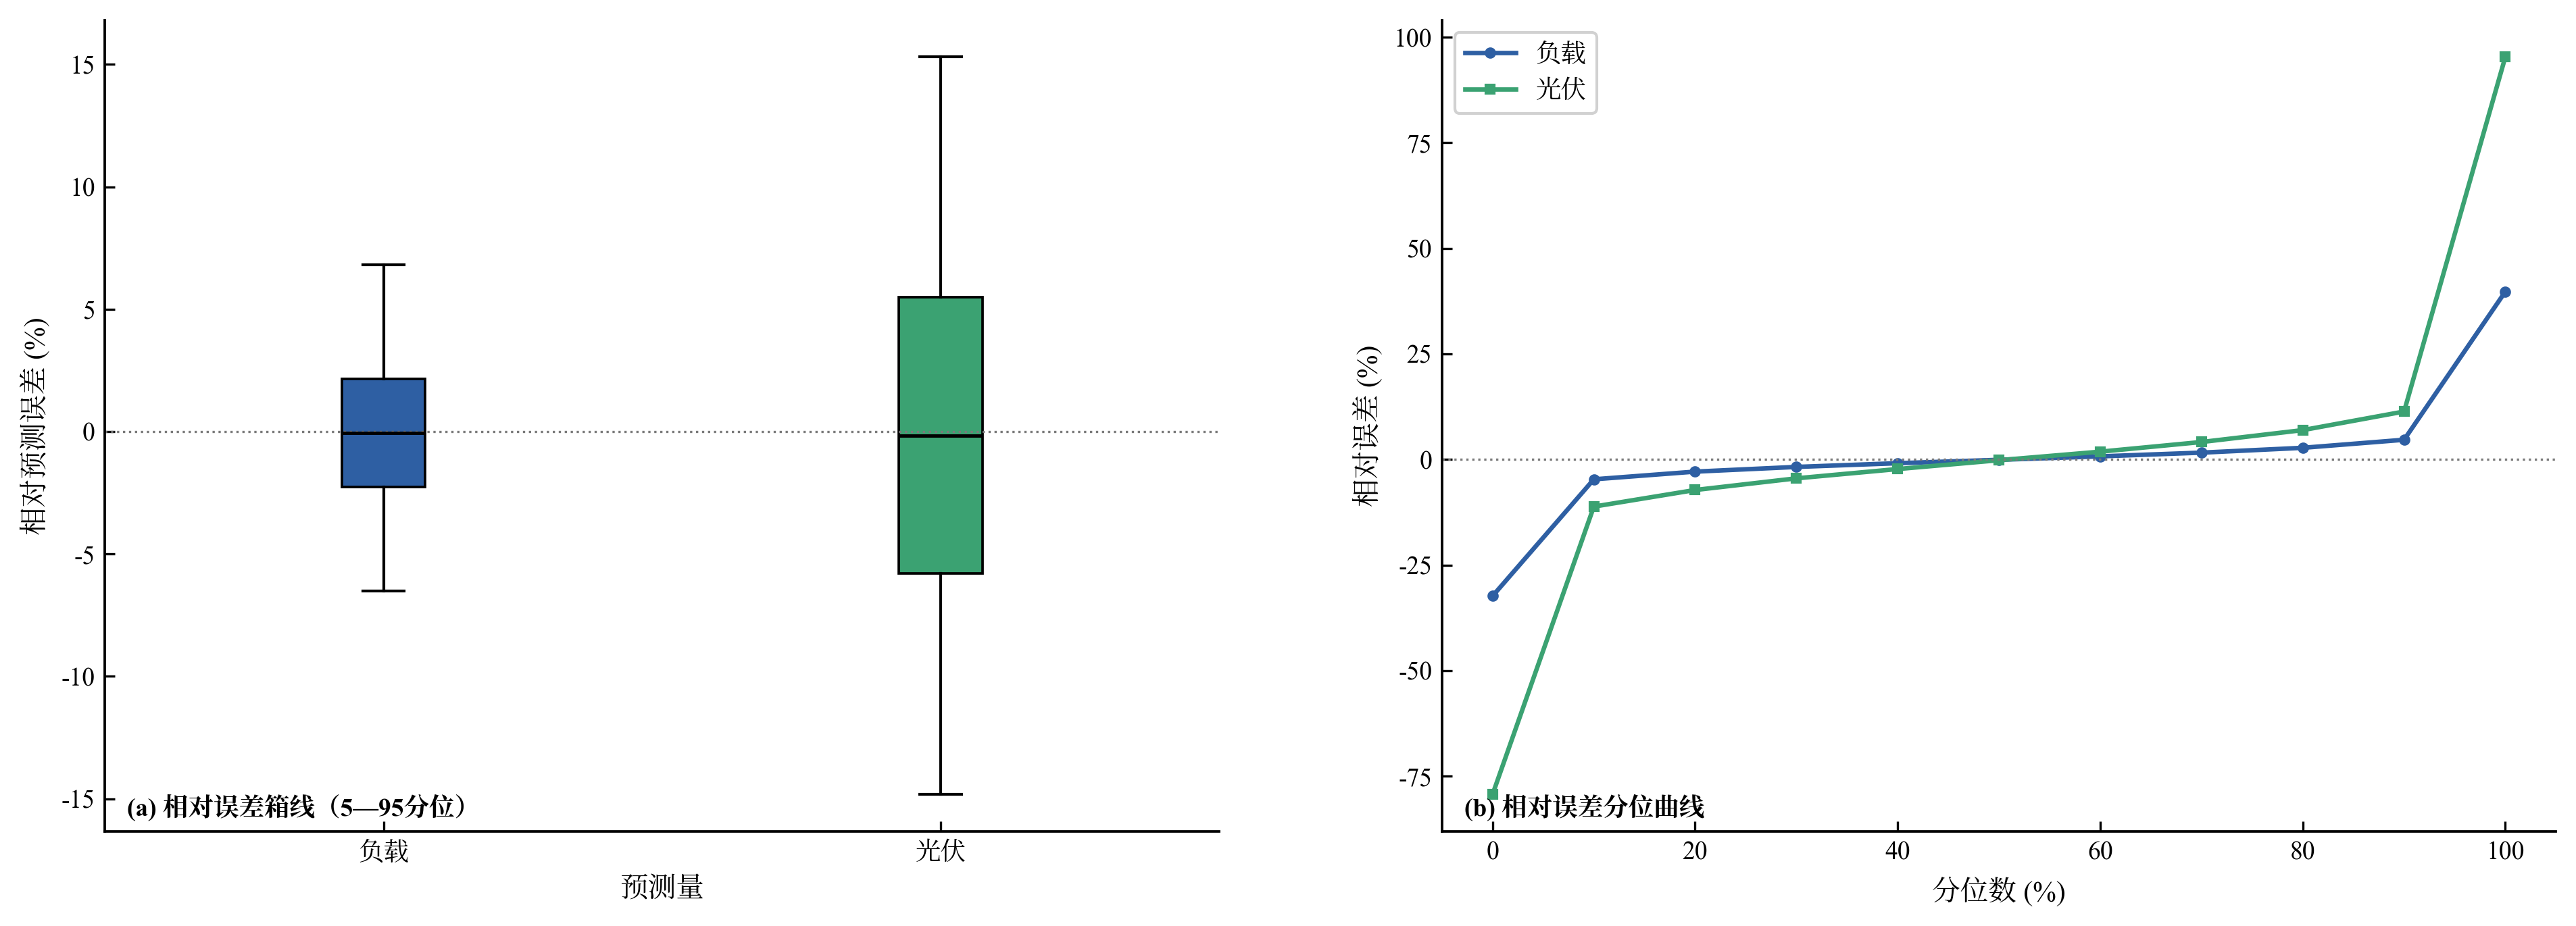
\includegraphics[width=0.78\textwidth]{求解/问题二/图片/图2-8_预测误差分布.png}
    \caption{负载与光伏预测相对误差的分布}
    \label{fig:结果2-8}
\end{figure}

\begin{longtable}{>{\centering\arraybackslash}p{0.15\textwidth}>{\centering\arraybackslash}p{0.13\textwidth}>{\centering\arraybackslash}p{0.15\textwidth}>{\centering\arraybackslash}p{0.13\textwidth}>{\centering\arraybackslash}p{0.15\textwidth}>{\centering\arraybackslash}p{0.13\textwidth}}
  \caption{2025.3.20 微网在指定时间段的购电量及全天的购电量和购电费}
  \label{tab:结果2-1a} \\
  \toprule
  时间段 & 购电量 & 时间段 & 购电量 & 时间段 & 购电量 \\
  \midrule
  \endfirsthead
  \caption{2025.3.20 微网在指定时间段的购电量及全天的购电量和购电费（续）} \\
  \toprule
  时间段 & 购电量 & 时间段 & 购电量 & 时间段 & 购电量 \\
  \midrule
  \endhead
  \bottomrule
  \endfoot
  10:00--10:10 & 0.00 & 12:00--12:10 & 535.11 & 14:00--14:10 & 0.00 \\
  16:00--16:10 & 506.24 & 18:00--18:10 & 712.75 & 20:00--20:10 & 0.00 \\
  全天购电量 & 68462.51 & 全天购电费 & 41502.92 &  &  \\
\end{longtable}

\begin{longtable}{>{\centering\arraybackslash}p{0.15\textwidth}>{\centering\arraybackslash}p{0.13\textwidth}>{\centering\arraybackslash}p{0.15\textwidth}>{\centering\arraybackslash}p{0.13\textwidth}>{\centering\arraybackslash}p{0.15\textwidth}>{\centering\arraybackslash}p{0.13\textwidth}}
  \caption{2025.6.21 微网在指定时间段的购电量及全天的购电量和购电费}
  \label{tab:结果2-1b} \\
  \toprule
  时间段 & 购电量 & 时间段 & 购电量 & 时间段 & 购电量 \\
  \midrule
  \endfirsthead
  \caption{2025.6.21 微网在指定时间段的购电量及全天的购电量和购电费（续）} \\
  \toprule
  时间段 & 购电量 & 时间段 & 购电量 & 时间段 & 购电量 \\
  \midrule
  \endhead
  \bottomrule
  \endfoot
  10:00--10:10 & 0.00 & 12:00--12:10 & 0.00 & 14:00--14:10 & 0.00 \\
  16:00--16:10 & 159.03 & 18:00--18:10 & 0.00 & 20:00--20:10 & 0.00 \\
  全天购电量 & 34663.14 & 全天购电费 & 19596.21 &  &  \\
\end{longtable}

\begin{longtable}{>{\centering\arraybackslash}p{0.15\textwidth}>{\centering\arraybackslash}p{0.13\textwidth}>{\centering\arraybackslash}p{0.15\textwidth}>{\centering\arraybackslash}p{0.13\textwidth}>{\centering\arraybackslash}p{0.15\textwidth}>{\centering\arraybackslash}p{0.13\textwidth}}
  \caption{2025.9.23 微网在指定时间段的购电量及全天的购电量和购电费}
  \label{tab:结果2-1c} \\
  \toprule
  时间段 & 购电量 & 时间段 & 购电量 & 时间段 & 购电量 \\
  \midrule
  \endfirsthead
  \caption{2025.9.23 微网在指定时间段的购电量及全天的购电量和购电费（续）} \\
  \toprule
  时间段 & 购电量 & 时间段 & 购电量 & 时间段 & 购电量 \\
  \midrule
  \endhead
  \bottomrule
  \endfoot
  10:00--10:10 & 0.00 & 12:00--12:10 & 528.89 & 14:00--14:10 & 0.00 \\
  16:00--16:10 & 561.39 & 18:00--18:10 & 807.53 & 20:00--20:10 & 11.96 \\
  全天购电量 & 72005.67 & 全天购电费 & 44887.63 &  &  \\
\end{longtable}

\begin{longtable}{>{\centering\arraybackslash}p{0.15\textwidth}>{\centering\arraybackslash}p{0.13\textwidth}>{\centering\arraybackslash}p{0.15\textwidth}>{\centering\arraybackslash}p{0.13\textwidth}>{\centering\arraybackslash}p{0.15\textwidth}>{\centering\arraybackslash}p{0.13\textwidth}}
  \caption{2025.12.21 微网在指定时间段的购电量及全天的购电量和购电费}
  \label{tab:结果2-1d} \\
  \toprule
  时间段 & 购电量 & 时间段 & 购电量 & 时间段 & 购电量 \\
  \midrule
  \endfirsthead
  \caption{2025.12.21 微网在指定时间段的购电量及全天的购电量和购电费（续）} \\
  \toprule
  时间段 & 购电量 & 时间段 & 购电量 & 时间段 & 购电量 \\
  \midrule
  \endhead
  \bottomrule
  \endfoot
  10:00--10:10 & 0.00 & 12:00--12:10 & 954.41 & 14:00--14:10 & 0.00 \\
  16:00--16:10 & 844.76 & 18:00--18:10 & 742.25 & 20:00--20:10 & 0.00 \\
  全天购电量 & 98496.73 & 全天购电费 & 63507.75 &  &  \\
\end{longtable}

2.1—12.31 逐日购电费用及其 7 日滑动平均如图\ref{fig:结果2-2}所示。可以看出，购电费呈现明显的季节性波动：冬季（12 月）因光伏出力低、负荷高，购电费最高；夏季（6 月）因光伏出力充沛，购电费最低，与光伏资源的季节规律一致。

\begin{figure}[H]
    \centering
    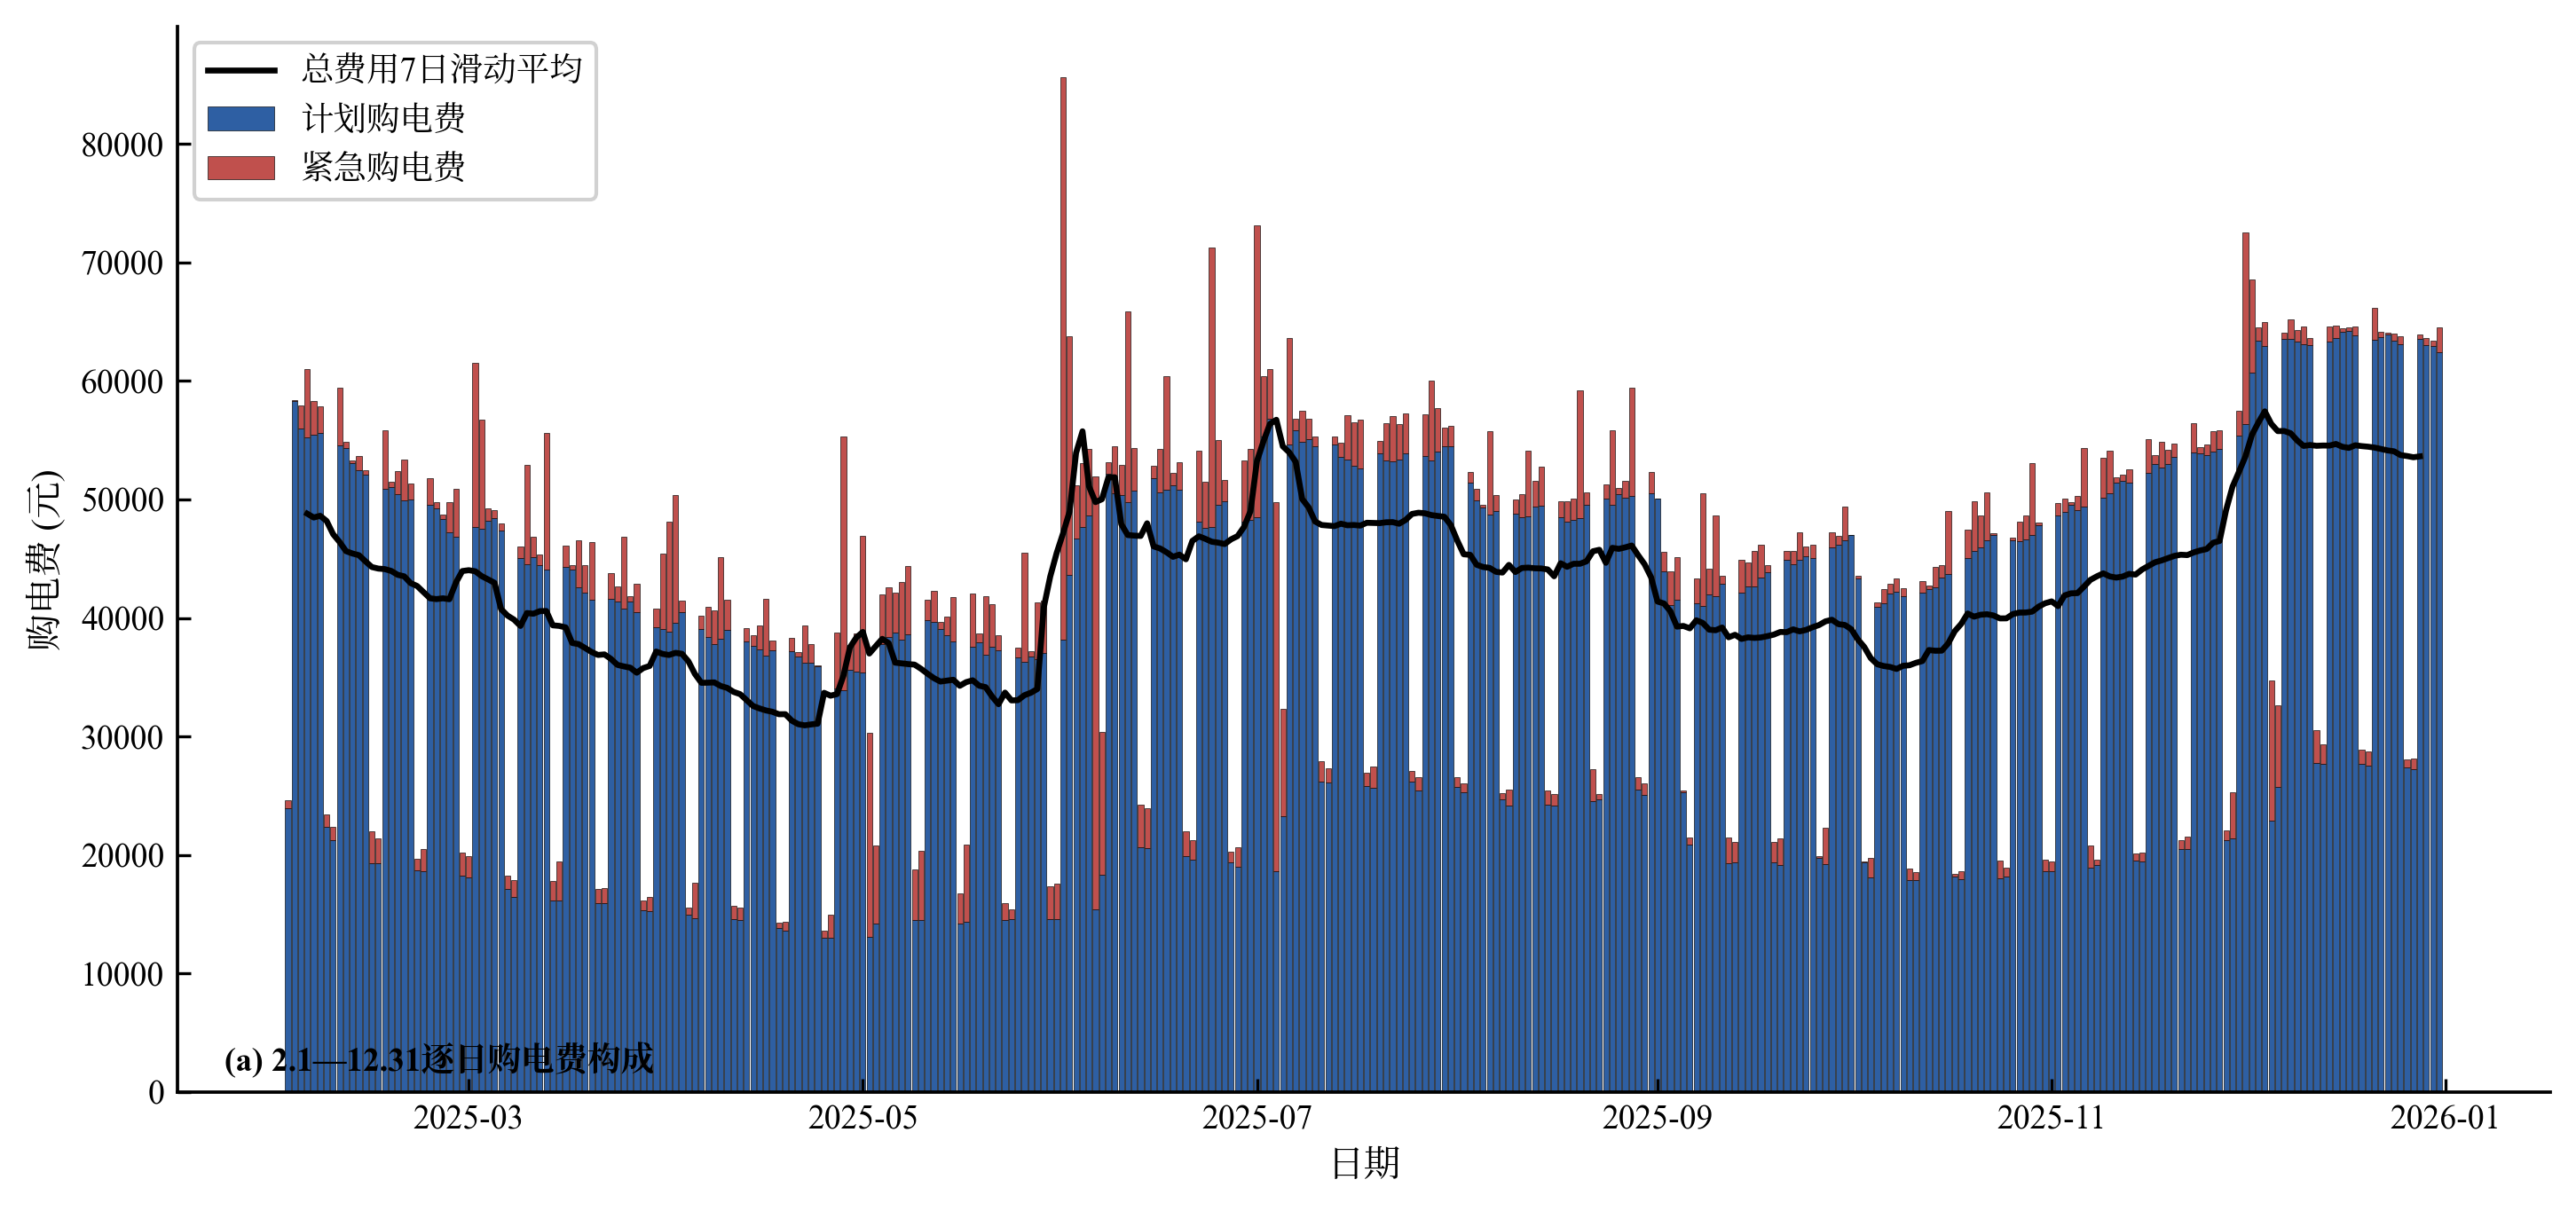
\includegraphics[width=0.70\textwidth]{求解/问题二/图片/图2-2_全年逐日购电费.png}
    \caption{2.1—12.31逐日购电费及7日滑动平均}
    \label{fig:结果2-2}
\end{figure}

四季典型日的购电功率曲线如图\ref{fig:结果2-3}所示。四个季节的购电功率均集中在夜间低电价时段，白天因光伏与储能放电的支撑，购电功率显著减小；冬季典型日购电功率整体最高，与表\ref{tab:结果2-1d}中冬季购电费最高相吻合。

\begin{figure}[H]
    \centering
    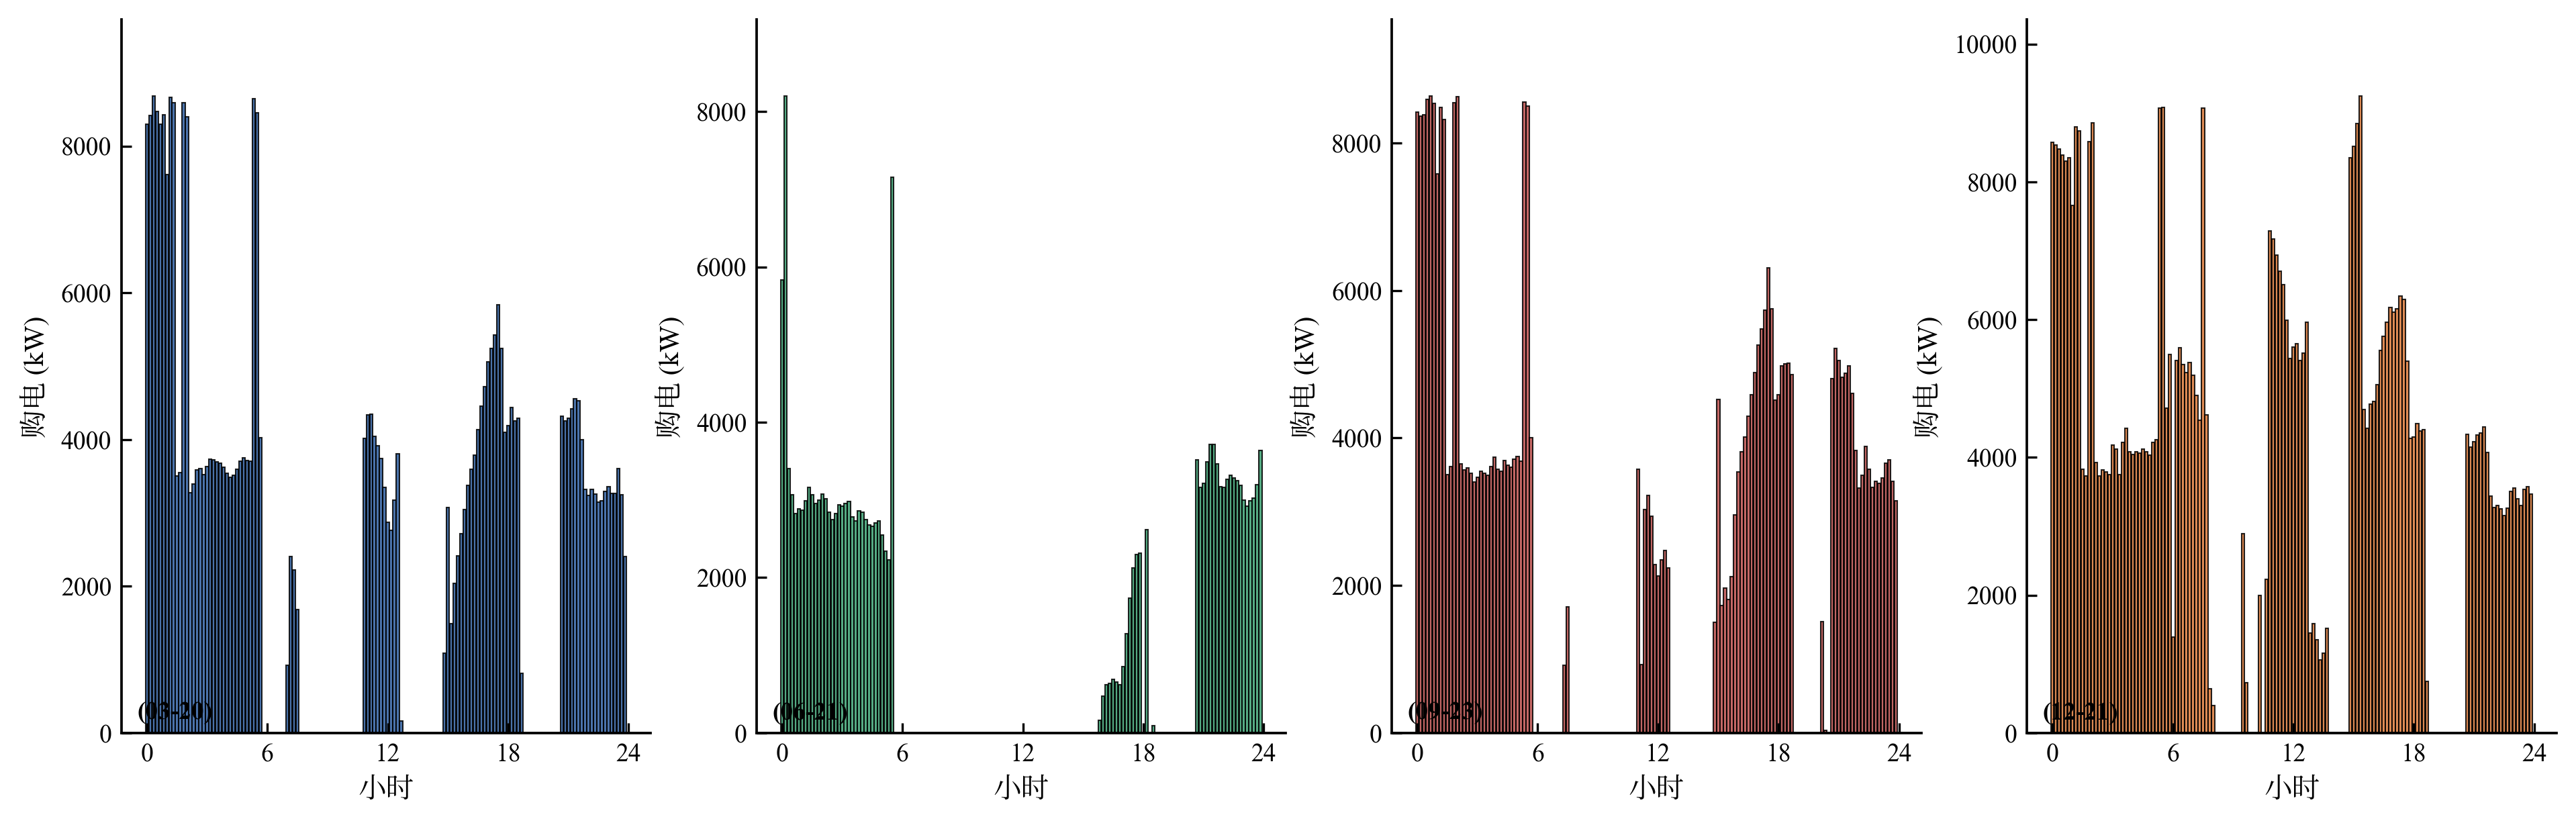
\includegraphics[width=0.75\textwidth]{求解/问题二/图片/图2-3_四季典型日购电策略.png}
    \caption{四季典型日的购电功率策略}
    \label{fig:结果2-3}
\end{figure}

四个指定日期的储能充放电结果如表\ref{tab:结果2-2a}$\sim$表\ref{tab:结果2-2d}所示。四日 0:00 与 24:00 储电量均回到 1200 kWh 下限，全天在 1200$\sim$10800 kWh 之间完成一次充放循环：00:00—04:00 与午间光伏富余时段充电，04:00—08:00 及 16:00—24:00 放电。四日 16:00—20:00 与 20:00—24:00 的放电量合计均为 8640 kWh，即 $0.9\times(10800-1200)$，说明每日晚间放出的电量恰好等于当日可用的储电量上限，“谷充峰放”被完全用尽。

\begin{longtable}{>{\centering\arraybackslash}p{0.15\textwidth}>{\centering\arraybackslash}p{0.13\textwidth}>{\centering\arraybackslash}p{0.13\textwidth}>{\centering\arraybackslash}p{0.15\textwidth}>{\centering\arraybackslash}p{0.13\textwidth}>{\centering\arraybackslash}p{0.13\textwidth}}
  \caption{2025.3.20 储能设备在指定时间段的充放电量及0:00和24:00的储电量}
  \label{tab:结果2-2a} \\
  \toprule
  时间段 & 充电量 & 放电量 & 时间段 & 充电量 & 放电量 \\
  \midrule
  \endfirsthead
  \caption{2025.3.20 储能设备在指定时间段的充放电量及0:00和24:00的储电量（续）} \\
  \toprule
  时间段 & 充电量 & 放电量 & 时间段 & 充电量 & 放电量 \\
  \midrule
  \endhead
  \bottomrule
  \endfoot
  0:00--4:00 & 9000.00 & 0.00 & 4:00--8:00 & 1666.67 & 5880.87 \\
  8:00--12:00 & 6050.98 & 2759.13 & 12:00--16:00 & 5029.62 & 335.29 \\
  16:00--20:00 & 0.00 & 5681.54 & 20:00--24:00 & 0.00 & 2958.46 \\
  0:00储电量 & 1200.00 &  & 24:00储电量 & 1200.00 &  \\
\end{longtable}

\begin{longtable}{>{\centering\arraybackslash}p{0.15\textwidth}>{\centering\arraybackslash}p{0.13\textwidth}>{\centering\arraybackslash}p{0.13\textwidth}>{\centering\arraybackslash}p{0.15\textwidth}>{\centering\arraybackslash}p{0.13\textwidth}>{\centering\arraybackslash}p{0.13\textwidth}}
  \caption{2025.6.21 储能设备在指定时间段的充放电量及0:00和24:00的储电量}
  \label{tab:结果2-2b} \\
  \toprule
  时间段 & 充电量 & 放电量 & 时间段 & 充电量 & 放电量 \\
  \midrule
  \endfirsthead
  \caption{2025.6.21 储能设备在指定时间段的充放电量及0:00和24:00的储电量（续）} \\
  \toprule
  时间段 & 充电量 & 放电量 & 时间段 & 充电量 & 放电量 \\
  \midrule
  \endhead
  \bottomrule
  \endfoot
  0:00--4:00 & 1857.78 & 0.00 & 4:00--8:00 & 862.32 & 2179.80 \\
  8:00--12:00 & 6229.23 & 0.00 & 12:00--16:00 & 4408.45 & 0.00 \\
  16:00--20:00 & 0.00 & 6124.20 & 20:00--24:00 & 0.00 & 2515.80 \\
  0:00储电量 & 1200.00 &  & 24:00储电量 & 1200.00 &  \\
\end{longtable}

\begin{longtable}{>{\centering\arraybackslash}p{0.15\textwidth}>{\centering\arraybackslash}p{0.13\textwidth}>{\centering\arraybackslash}p{0.13\textwidth}>{\centering\arraybackslash}p{0.15\textwidth}>{\centering\arraybackslash}p{0.13\textwidth}>{\centering\arraybackslash}p{0.13\textwidth}}
  \caption{2025.9.23 储能设备在指定时间段的充放电量及0:00和24:00的储电量}
  \label{tab:结果2-2c} \\
  \toprule
  时间段 & 充电量 & 放电量 & 时间段 & 充电量 & 放电量 \\
  \midrule
  \endfirsthead
  \caption{2025.9.23 储能设备在指定时间段的充放电量及0:00和24:00的储电量（续）} \\
  \toprule
  时间段 & 充电量 & 放电量 & 时间段 & 充电量 & 放电量 \\
  \midrule
  \endhead
  \bottomrule
  \endfoot
  0:00--4:00 & 9000.00 & 0.00 & 4:00--8:00 & 1666.67 & 5909.41 \\
  8:00--12:00 & 6150.33 & 2730.59 & 12:00--16:00 & 4809.30 & 237.30 \\
  16:00--20:00 & 0.00 & 5811.32 & 20:00--24:00 & 0.00 & 2828.68 \\
  0:00储电量 & 1200.00 &  & 24:00储电量 & 1200.00 &  \\
\end{longtable}

\begin{longtable}{>{\centering\arraybackslash}p{0.15\textwidth}>{\centering\arraybackslash}p{0.13\textwidth}>{\centering\arraybackslash}p{0.13\textwidth}>{\centering\arraybackslash}p{0.15\textwidth}>{\centering\arraybackslash}p{0.13\textwidth}>{\centering\arraybackslash}p{0.13\textwidth}}
  \caption{2025.12.21 储能设备在指定时间段的充放电量及0:00和24:00的储电量}
  \label{tab:结果2-2d} \\
  \toprule
  时间段 & 充电量 & 放电量 & 时间段 & 充电量 & 放电量 \\
  \midrule
  \endfirsthead
  \caption{2025.12.21 储能设备在指定时间段的充放电量及0:00和24:00的储电量（续）} \\
  \toprule
  时间段 & 充电量 & 放电量 & 时间段 & 充电量 & 放电量 \\
  \midrule
  \endhead
  \bottomrule
  \endfoot
  0:00--4:00 & 9000.00 & 0.00 & 4:00--8:00 & 2500.00 & 1508.33 \\
  8:00--12:00 & 5833.33 & 7806.67 & 12:00--16:00 & 8160.87 & 2695.30 \\
  16:00--20:00 & 0.00 & 5609.21 & 20:00--24:00 & 0.00 & 3030.79 \\
  0:00储电量 & 1200.00 &  & 24:00储电量 & 1200.00 &  \\
\end{longtable}

四季典型日的储能荷电状态轨迹如图\ref{fig:结果2-4}所示。储能荷电状态每日在 1200 kWh 与 10800 kWh 之间完成一次充放循环，白天光伏盈余时充电、夜间与傍晚放电，且全天严格处于约束区间内，验证了滚动模型与日末状态传递机制的可行性。

\begin{figure}[H]
    \centering
    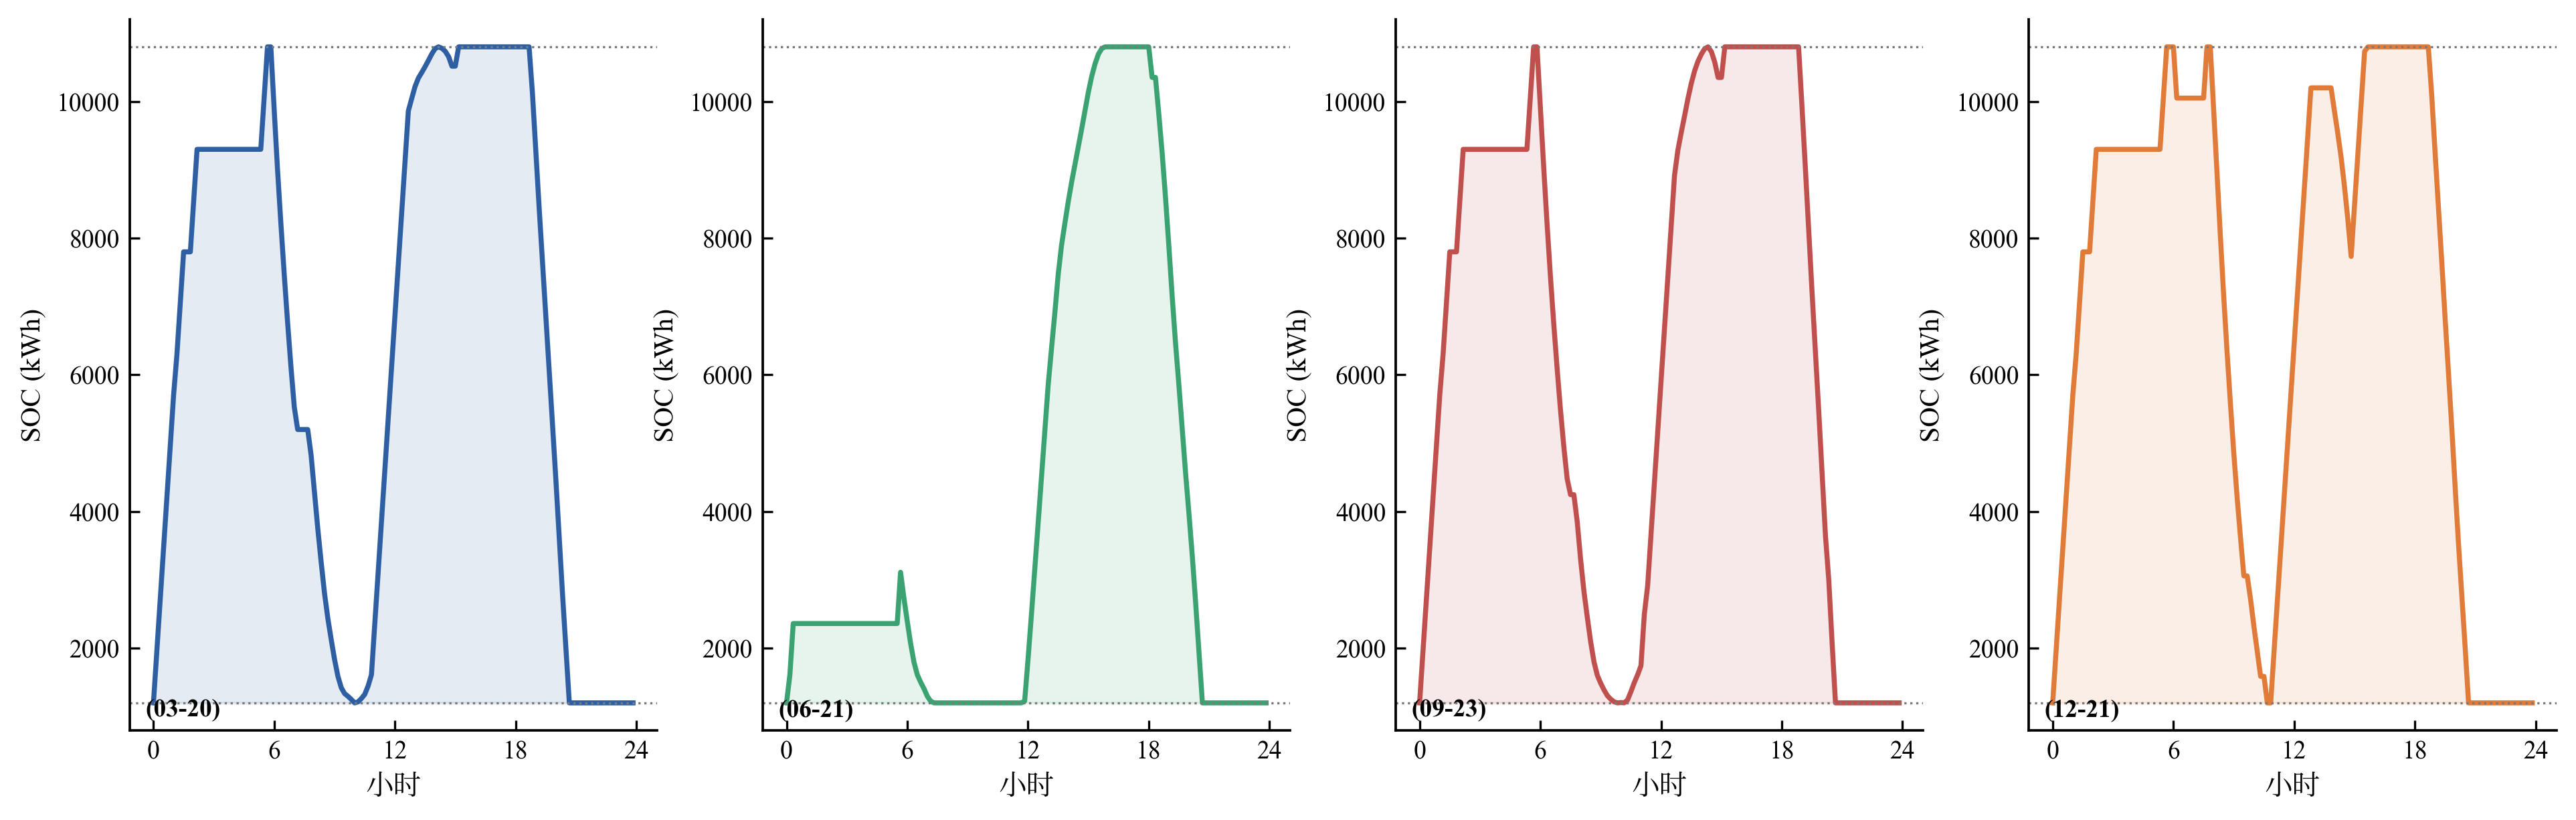
\includegraphics[width=0.75\textwidth]{求解/问题二/图片/图2-4_四季典型日SOC轨迹.png}
    \caption{四季典型日储能荷电状态轨迹}
    \label{fig:结果2-4}
\end{figure}

2—12 月储能每日 0:00 储电量的月度分布如图\ref{fig:结果2-5}所示。各月储电量中位数均处于 1200 kWh 下限附近。由于每日电价相同、跨日留存电量还需额外承担约 $19\%$ 的往返损耗，日间不存在跨日套利空间，故日末储电量必然放至下限；本图与这一理论推断完全吻合，说明日内低充高放套利已被充分利用，而非模型的人为约束所致。

\begin{figure}[H]
    \centering
    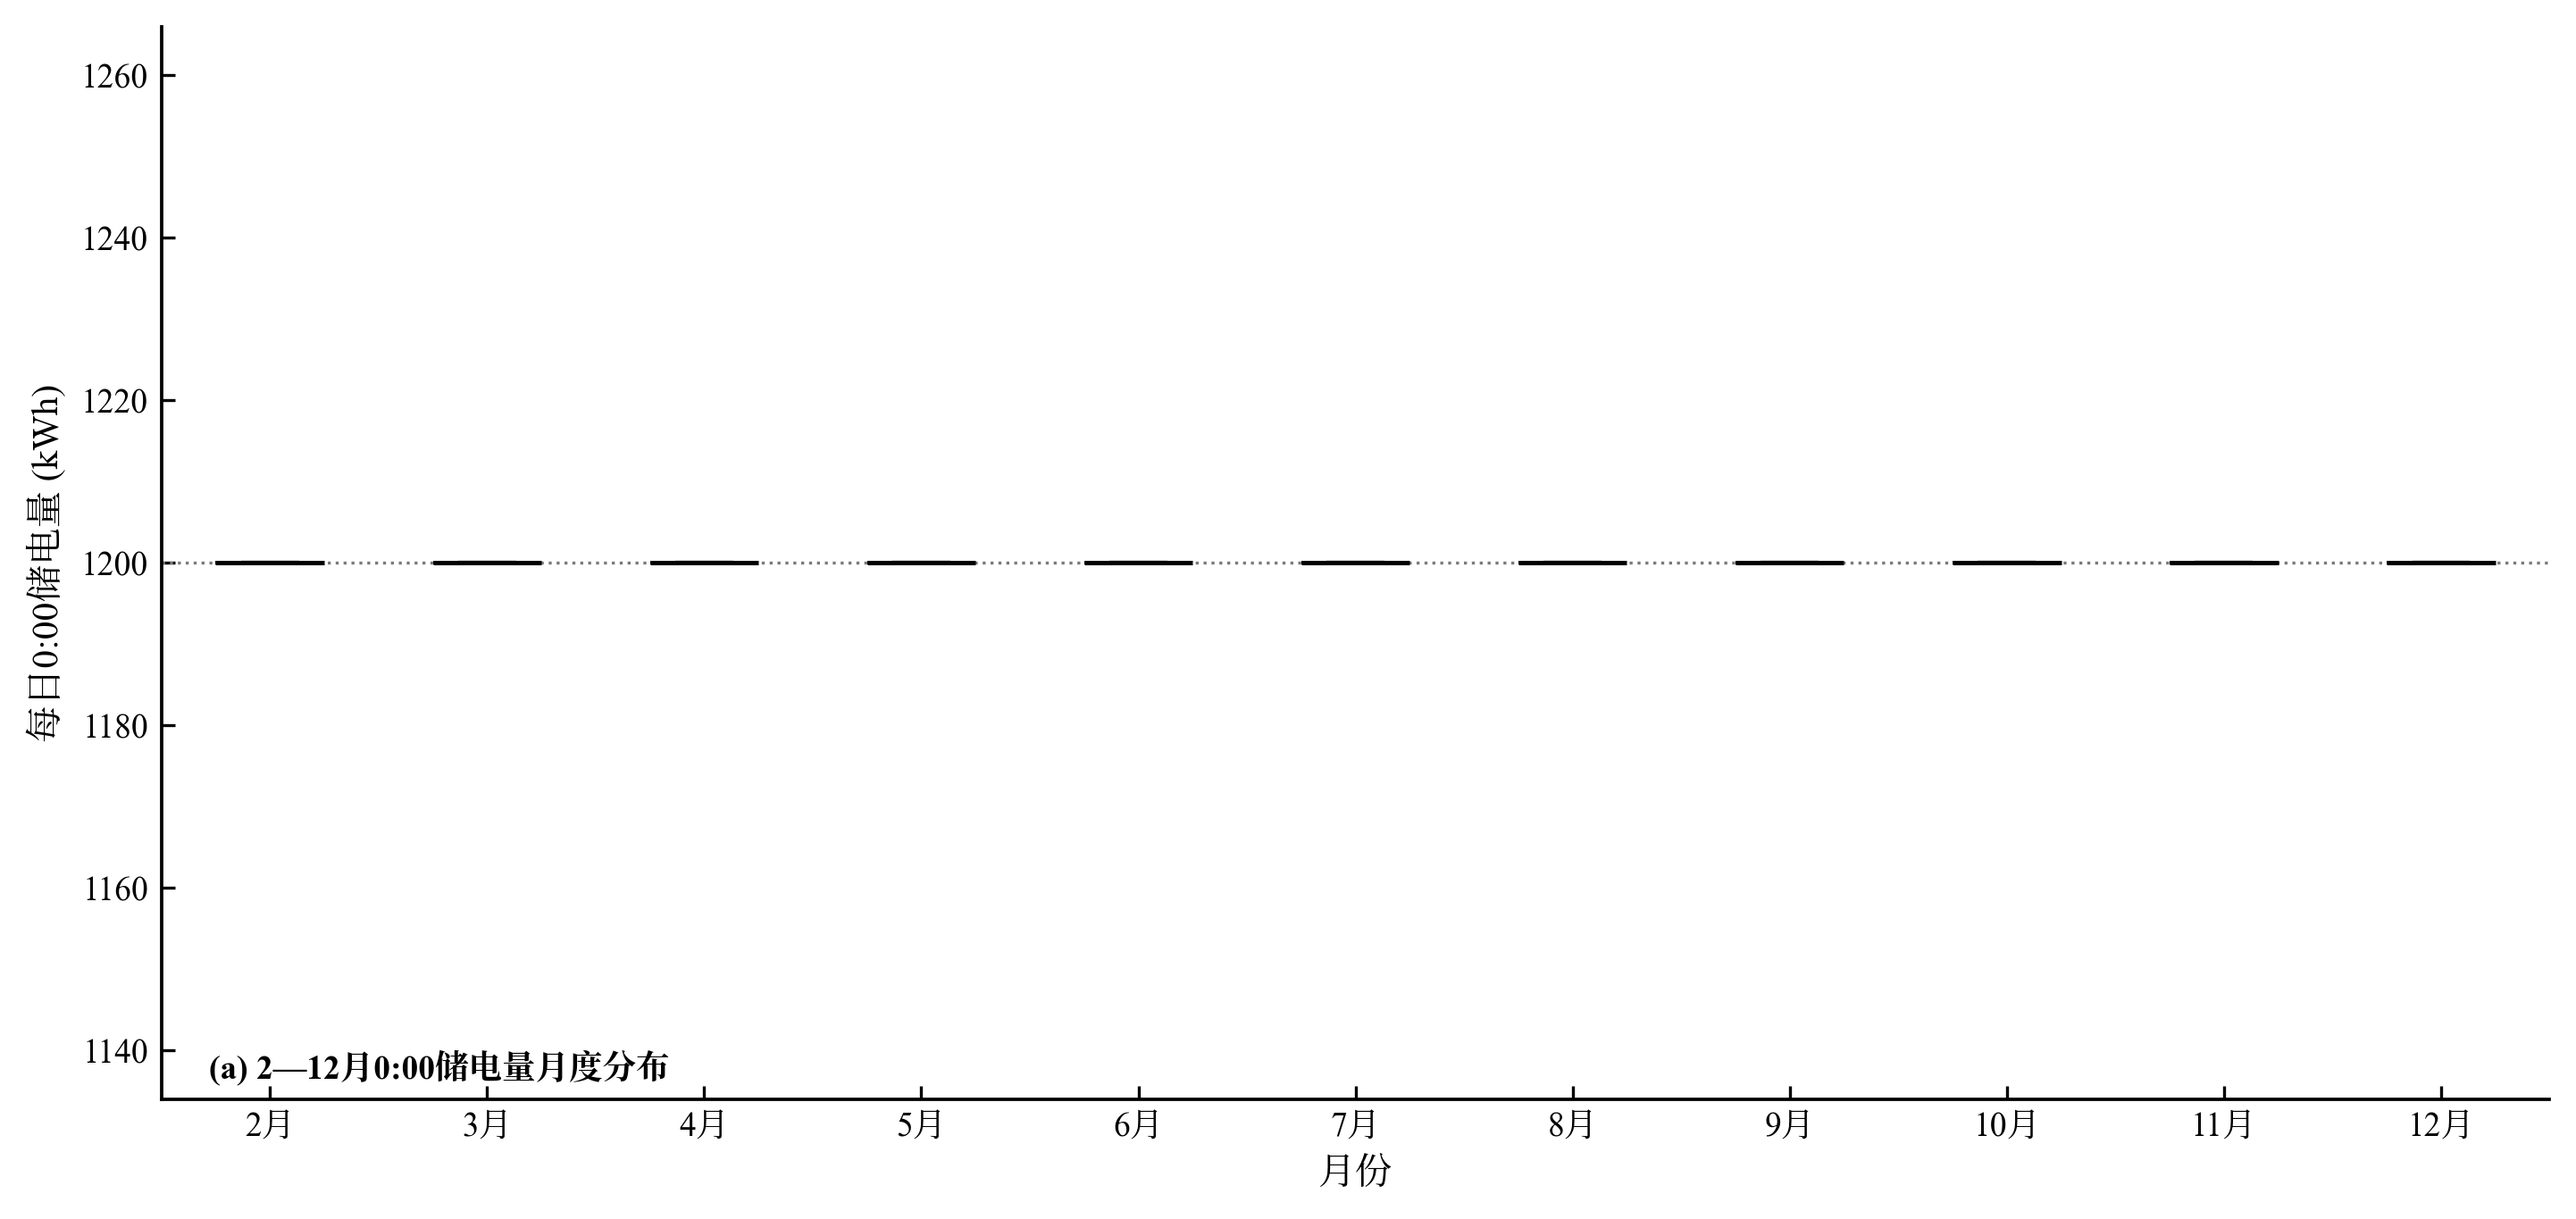
\includegraphics[width=0.70\textwidth]{求解/问题二/图片/图2-5_全年储能SOC月度分布.png}
    \caption{储能每日0:00储电量月度分布（2—12月）}
    \label{fig:结果2-5}
\end{figure}

紧急购电的分段明细如表\ref{tab:结果2-3}所示。四个指定日期分别出现 16、11、15、10 段紧急购电，合计分别为 1400.66 kWh、424.89 kWh、583.54 kWh 和 830.33 kWh；单次连续段的时长多在 10$\sim$30 分钟之间，最长的单段为 12 月 21 日 10:20—11:40 的 608.79 kWh。从时段分布看，紧急购电集中在两类时刻：一是夜间与清晨（00:00—08:00）负荷预测偏低、而储能计划未安排放电的时段；二是傍晚（16:00—20:00）光伏出力衰减快于预测、储能放电已按计划结束的时段。图\ref{fig:结果2-9}进一步给出全年紧急购电功率的分布，可见其量级集中在 0$\sim$500 kW，且随月份变化，冬季整体高于夏季。

\begin{longtable}{>{\centering\arraybackslash}p{0.11\textwidth}>{\centering\arraybackslash}p{0.08\textwidth}>{\centering\arraybackslash}p{0.11\textwidth}>{\centering\arraybackslash}p{0.08\textwidth}>{\centering\arraybackslash}p{0.11\textwidth}>{\centering\arraybackslash}p{0.08\textwidth}>{\centering\arraybackslash}p{0.11\textwidth}>{\centering\arraybackslash}p{0.08\textwidth}}
  \caption{微网在指定日期的紧急购电量}
  \label{tab:结果2-3} \\
  \toprule
  \multicolumn{2}{c}{2025.3.20} & \multicolumn{2}{c}{2025.6.21} & \multicolumn{2}{c}{2025.9.23} & \multicolumn{2}{c}{2025.12.21} \\
  \cmidrule(lr){1-2} \cmidrule(lr){3-4} \cmidrule(lr){5-6} \cmidrule(lr){7-8}
  时间段 & 购电量 & 时间段 & 购电量 & 时间段 & 购电量 & 时间段 & 购电量 \\
  \midrule
  \endfirsthead
  \caption{微网在指定日期的紧急购电量（续）} \\
  \toprule
  \multicolumn{2}{c}{2025.3.20} & \multicolumn{2}{c}{2025.6.21} & \multicolumn{2}{c}{2025.9.23} & \multicolumn{2}{c}{2025.12.21} \\
  \cmidrule(lr){1-2} \cmidrule(lr){3-4} \cmidrule(lr){5-6} \cmidrule(lr){7-8}
  时间段 & 购电量 & 时间段 & 购电量 & 时间段 & 购电量 & 时间段 & 购电量 \\
  \midrule
  \endhead
  \bottomrule
  \endfoot
  00:20--00:30 & 19.84 & 00:00--00:30 & 85.44 & 05:00--05:10 & 2.37 & 03:00--03:10 & 9.16 \\
  01:00--01:30 & 15.95 & 01:20--01:40 & 39.32 & 05:40--05:50 & 0.16 & 03:30--03:50 & 47.74 \\
  03:10--03:30 & 10.22 & 02:00--02:20 & 15.39 & 06:50--07:10 & 5.73 & 05:40--05:50 & 22.51 \\
  04:50--05:10 & 7.72 & 02:50--03:00 & 3.76 & 09:30--09:50 & 30.65 & 10:20--11:40 & 608.79 \\
  05:40--05:50 & 10.16 & 03:20--03:30 & 3.70 & 10:00--10:10 & 22.22 & 12:50--13:10 & 46.57 \\
  08:50--10:00 & 267.99 & 05:50--06:20 & 42.33 & 10:50--11:00 & 27.63 & 15:20--15:30 & 6.95 \\
  10:50--12:00 & 469.05 & 17:30--17:50 & 4.97 & 14:20--15:30 & 368.13 & 17:20--17:30 & 21.30 \\
  12:30--12:50 & 139.73 & 18:50--19:10 & 86.14 & 16:00--16:20 & 53.52 & 19:50--20:00 & 34.91 \\
  14:10--14:20 & 6.87 & 20:20--20:40 & 44.73 & 16:30--16:40 & 1.67 & 22:50--23:00 & 20.49 \\
  14:40--15:00 & 15.60 & 21:20--21:30 & 1.47 & 17:00--17:10 & 9.35 & 23:40--00:00 & 11.91 \\
  15:10--17:10 & 327.28 & 21:50--23:00 & 97.65 & 18:30--18:40 & 2.86 &  &  \\
  18:40--19:10 & 32.59 &  &  & 20:10--20:30 & 5.84 &  &  \\
  20:00--20:20 & 36.03 &  &  & 20:50--21:00 & 24.00 &  &  \\
  21:20--21:30 & 7.01 &  &  & 21:50--22:00 & 9.28 &  &  \\
  22:50--23:00 & 6.53 &  &  & 22:20--22:30 & 20.13 &  &  \\
  23:30--23:40 & 28.08 &  &  &  &  &  &  \\
  合计 & 1400.66 & 合计 & 424.89 & 合计 & 583.54 & 合计 & 830.33 \\
\end{longtable}

\begin{figure}[H]
    \centering
    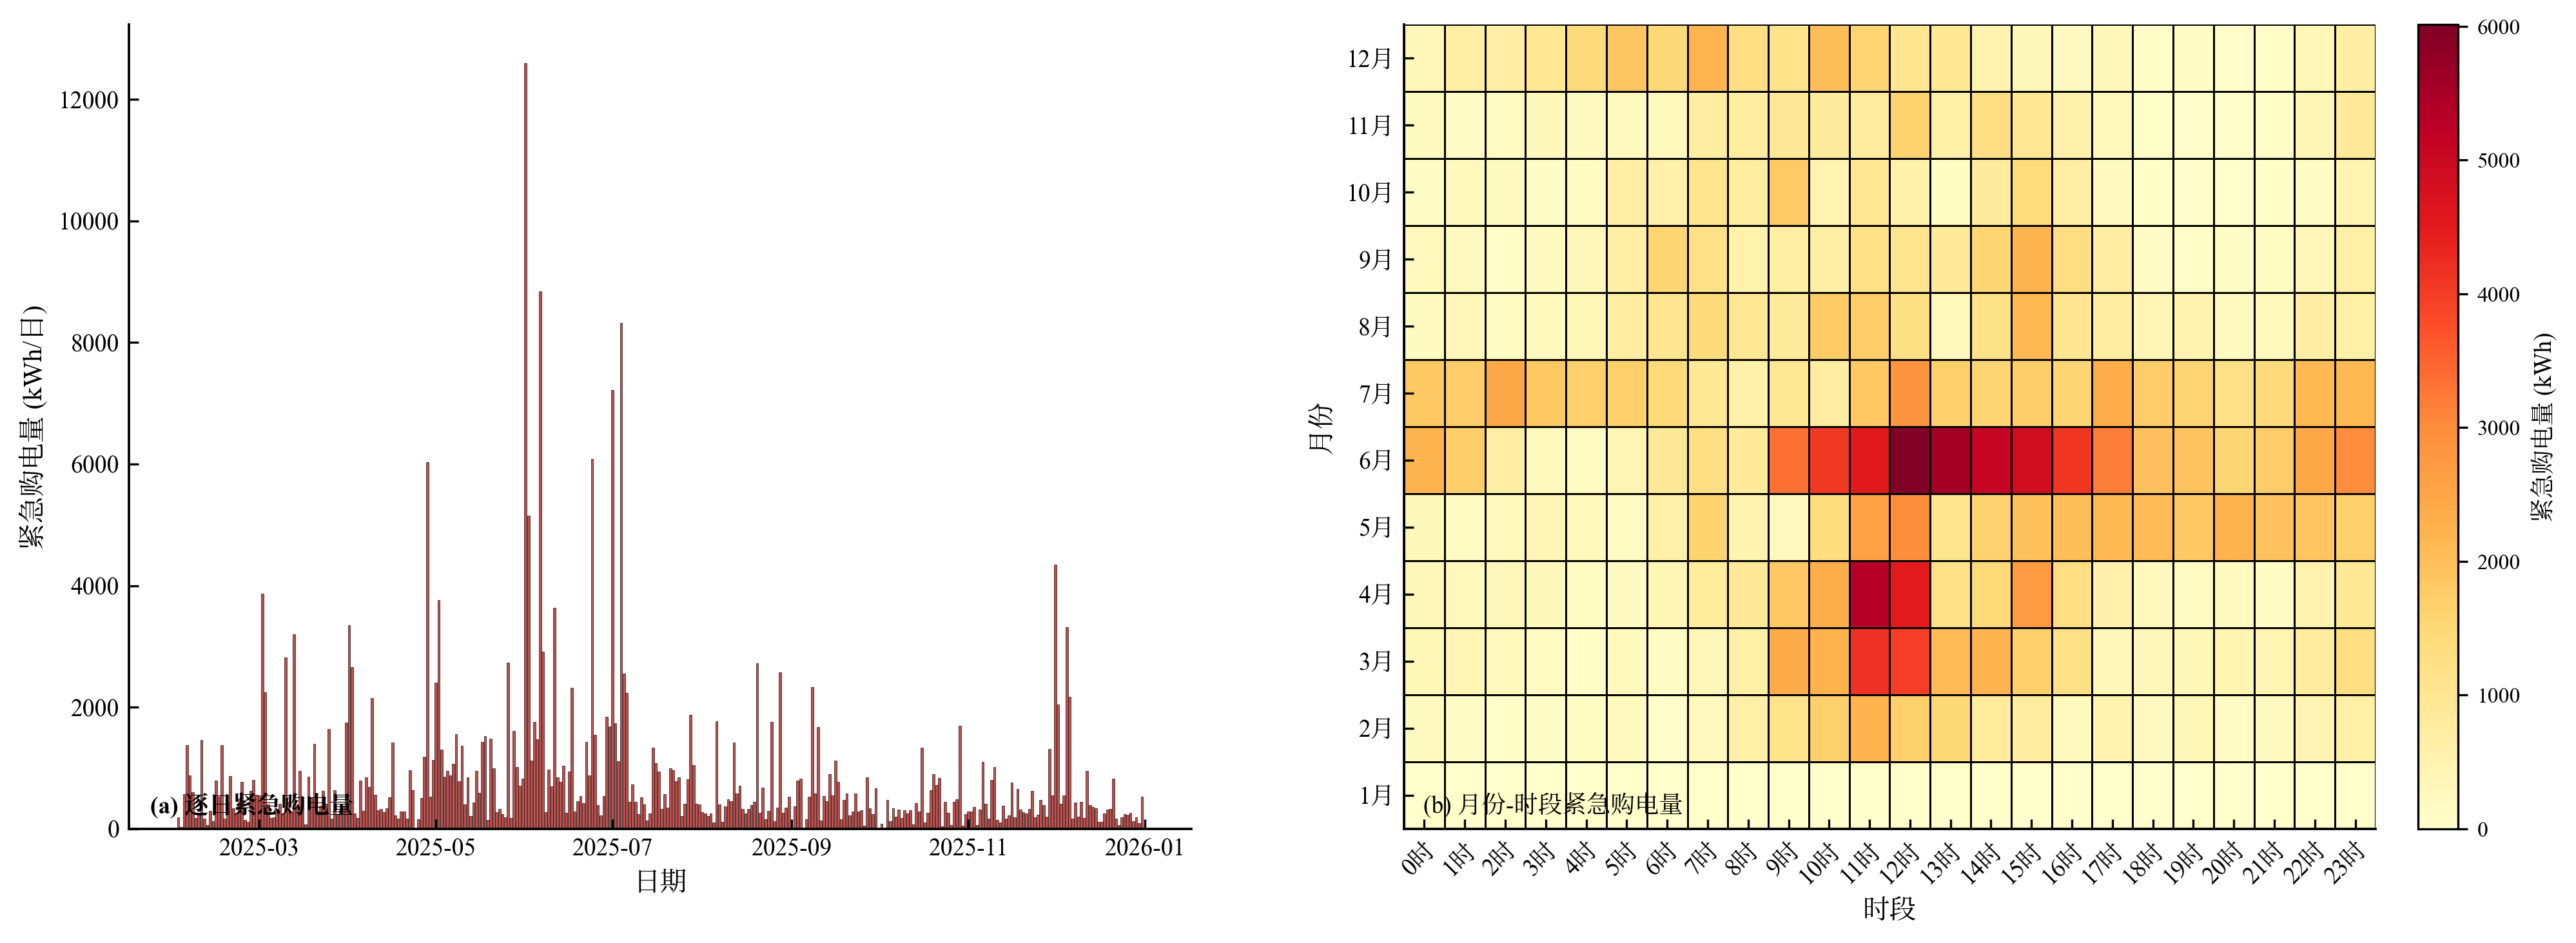
\includegraphics[width=0.78\textwidth]{求解/问题二/图片/图2-9_紧急购电分布.png}
    \caption{全年紧急购电量的分布}
    \label{fig:结果2-9}
\end{figure}

购电功率与净负荷的关系（2.1—12.31）及月度购电费（2—12月）如图\ref{fig:结果2-6}所示。日均购电功率与日均净负荷呈显著正相关，负荷越大、光伏越小则购电越多；月度购电费在冬季达到峰值、夏季为谷值，进一步印证了模型的合理性。

\begin{figure}[H]
    \centering
    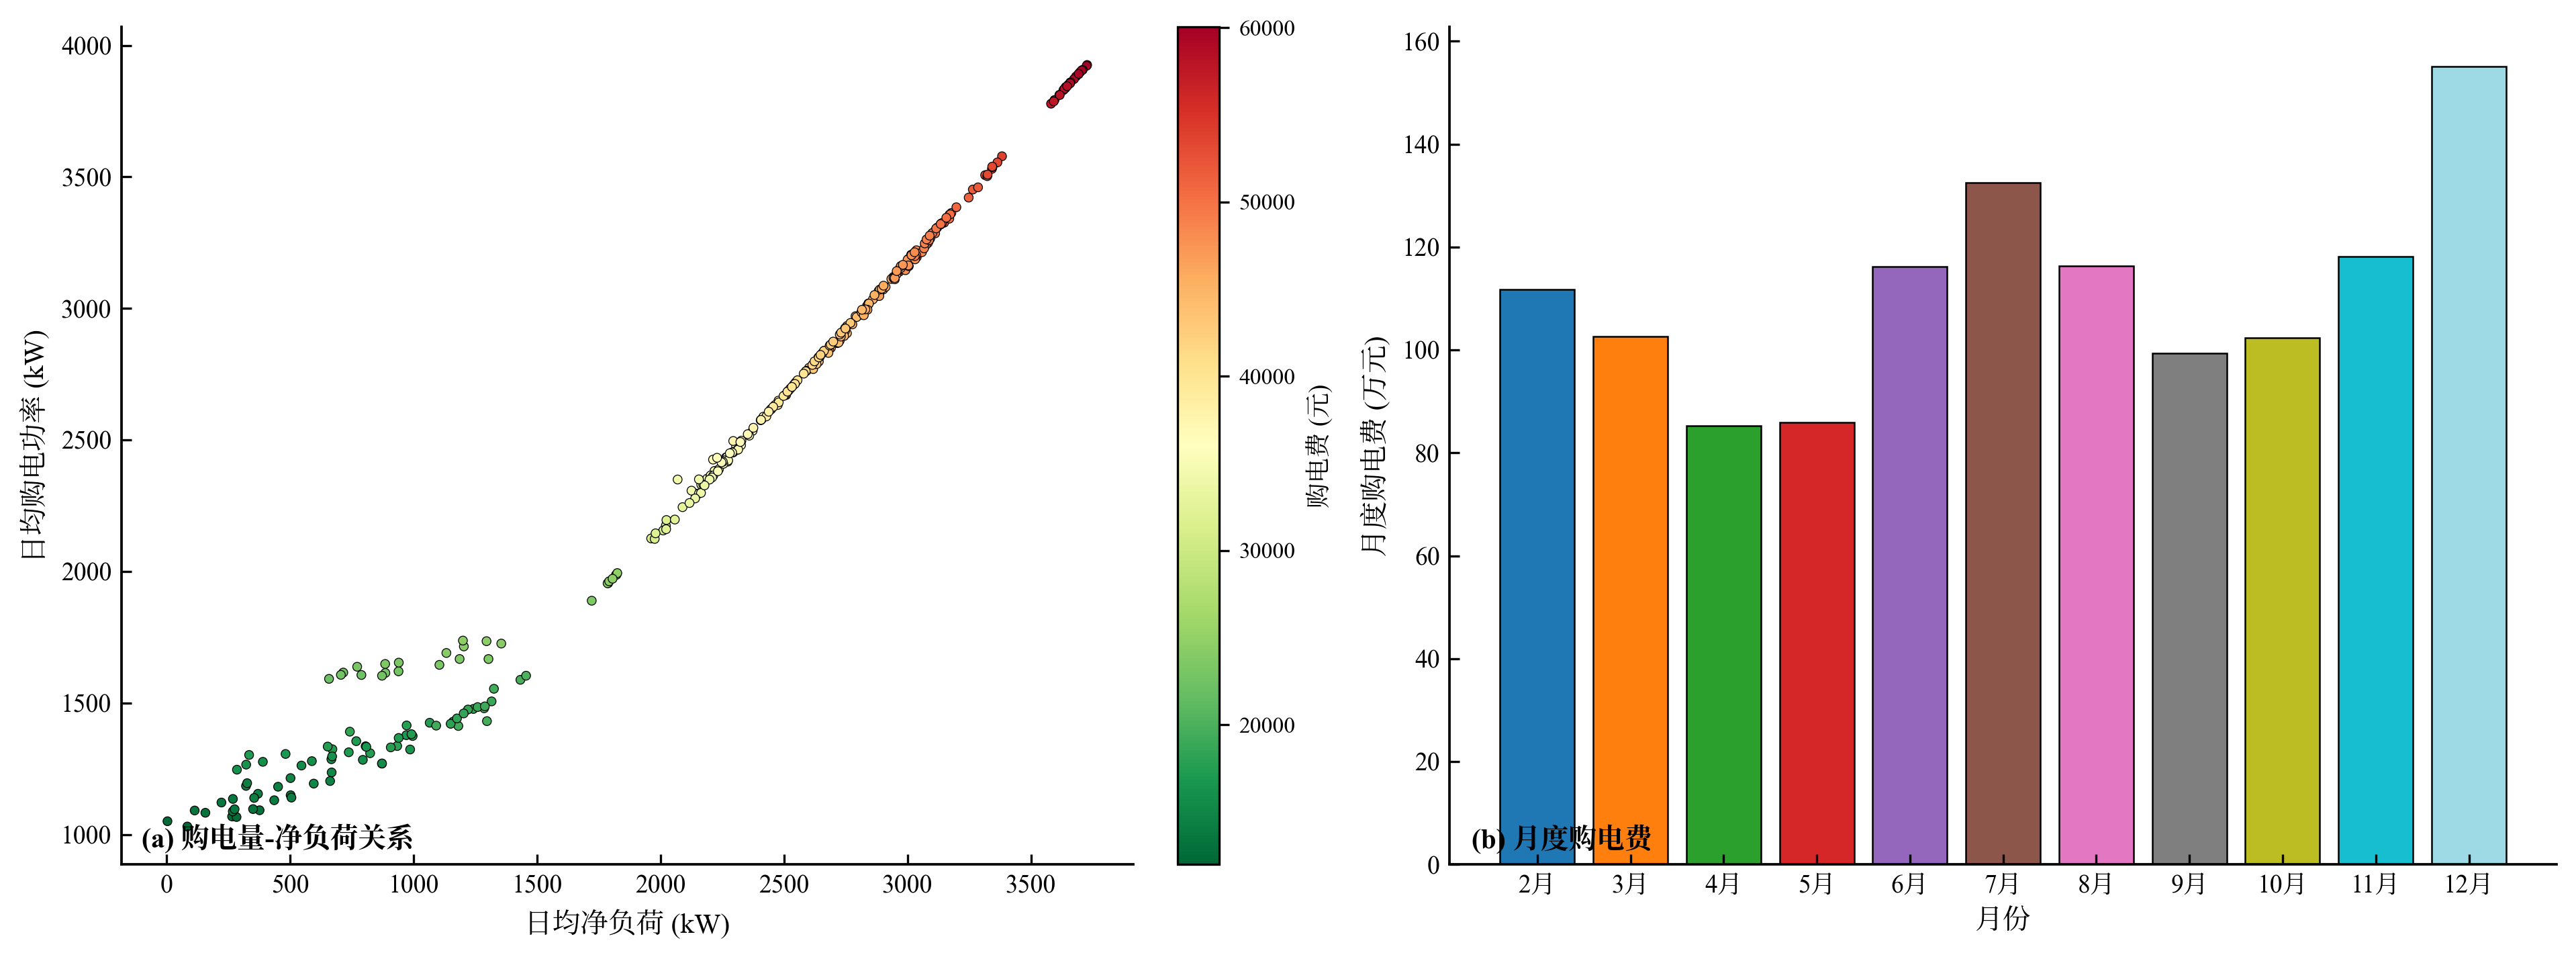
\includegraphics[width=0.72\textwidth]{求解/问题二/图片/图2-6_购电量与净负荷关系.png}
    \caption{购电功率与净负荷的关系及月度购电费}
    \label{fig:结果2-6}
\end{figure}

全年调度方案的收支可以由两条独立的账目互相印证。334 天净负荷合计 17939189.49 kWh，储能放电 5520412.99 kWh、充电 6815324.68 kWh，计划购电与紧急购电共同满足用电需求；计划段与紧急段之间的能量平衡校验为“净负荷$-$计划购电量$-$放电量$+$充电量$=-2598964.74$ kWh”，恰等于“紧急购电量 282910.68 kWh 减弃电量 2881875.41 kWh”，表明逐日结算无遗漏。另一方面，弃电量合计 2881875.41 kWh 主要来自午间光伏超发：光伏出力峰值可达 10216.2 kW，高于负荷峰值 7978.9 kW，储能充满后富余电力无处消纳，其中约三分之二来自光伏侧，其余为光伏超出预测时计划购电形成的少量富余。与弃电相反，紧急购电集中在夜间与傍晚光伏不足时段，334 天中 333 天出现、覆盖 17.90\% 的间隔，说明预测偏差由 5 倍电价兜底，而非被事后信息抹平。
